\chapter{\large Fundamentación teórica}

\pagestyle{fancy}
\lhead{}
\chead{}
\rhead{Capítulo 1: Fundamentación teórica}
\lfoot{}
\cfoot{}
\rfoot{\thepage}
\renewcommand{\headrulewidth}{0.4pt}
%\renewcommand{\footrulewidth}{0.4pt}
 \vspace{-1cm}

%\lettrine[lines=2, lraise=0, nindent=0em, slope=-.5em]
\section{Introducción}
sdfsdf
\section{Control de Autoridades}
El Control de Autoridades es un problema global que afecta a organizaciones de diversos tipos \citep{Leiva-Mederos2013}. La comunidad bibliotecaria durante largo tiempo ha sido consciente de la necesidad del Control de Autoridades \citep{Harper2007,Tillett2009,Leiva-Mederos2013,Carrasco2016}. La necesidad de almacenar uniformemente la información correspondiente a cada autor incluido en un catálogo es abordada en el trabajo y la investigación de varias organizaciones internacionales \citep{Leiva-Mederos2013}. Una panorámica breve del desarrollo en el Control de Autoridades incluiría los siguientes elementos:

\begin{itemize}
\item Se hace explícita la necesidad del Control de Autoridades y surge la ``Cooperación en Nombres de Autoridades'' (``Name Authority Cooperative'' - NACO, por sus siglas de acuerdo al término en idioma inglés) en la ``Biblioteca del Congreso'' (``Library of Congress'' - LOC, por sus siglas de acuerdo al término en idioma inglés) de los Estados Unidos de América \citep{Leiva-Mederos2013}. En Asia se establece el ``Nombre de Autoridad de Hong Kong Chino'' (``Hong Kong Chinese Authority Name'' - HKCAN, por sus siglas de acuerdo al término en idioma inglés). Esto significó el reconocimiento de la problemática por dos organizaciones internacionales a partir de los elementos enunciados en el siglo XIX por \cite{cutter1889rules}.

\item \cite{lubetzky1969principles} mejoran la búsqueda y recuperación de trabajos en catálogos bibliográficos.

\item \cite{bregzis1982syndetic} crea el ``Número Internacional Estandarizado de Datos de Autoridad'' (``International Standard Authority Data Number'' - ISADN, por sus siglas de acuerdo al término en idioma inglés) con el fin de vencer las dificultades al recuperar registros bibliográficos con trabajos relativos a un autor en específico y trabajos almacenados bajo un título uniforme.

\item La LOC crea el LC/NAF \citep{Sandberg2016}.

\item La IFLA crea los FRAD \citep{InternationalFederationofLibraryAssociationsandInstitutions2009}.

\item El ``Centro Bibliotecario Computarizado En Línea'' (``Online Computer Library Center'' - OCLC, por sus siglas de acuerdo al término en idioma inglés) crea el VIAF \citep{OCLCOnlineComputerLibraryCenterInc.2014}.
\end{itemize}

La necesidad de crear registros de autoridad de alta calidad ha impulsado la creación de herramientas como AUTHORIS \citep{Leiva-Mederos2013}. AUTHORIS aspira a facilitar el procesamiento de datos de autoridad en una manera estandarizada siguiendo los principios de los Datos Enlazados Abiertos \citep{Berners-Lee2006}.

\section{Web Semántica}
La Web 2.0 se basa en un conjunto de tecnologías y estándares definidos por el ``Consorcio World Wide Web'' (``World Wide Web Consortium'' - W3C, por sus siglas de acuerdo al término en idioma inglés) entre los que se encuentra el ``Protocolo de Transferencia de Hipertextos'' (``Hypertext Transfer Protocol'' - HTTP, por sus siglas de acuerdo al término en idioma inglés), los ``Identificadores de Recursos Universales'' (``Universal Resource Identifier'' - URI, por sus siglas de acuerdo al término en idioma inglés) y el ``Lenguaje de Marcado de Hipertextos'' (``Hypertext Markup Language'' - HTML, por sus siglas de acuerdo al término en idioma inglés) para la representación de contenidos \citep{Masinter2005}. Este último carece de un mecanismo para expresar el significado de los contenidos publicados, imposibilitando a las computadoras procesar los mismos automáticamente \citep{Hidalgo-Delgado2015}.

El significado del término Web Semántica es definido por \cite{Berners-Lee2001} en un artículo donde expresa: \textit{La Web Semántica no es una Web aparte, sino una extensión de la existente en la que la información posee significado formalmente definido, facilitando que las computadoras y los humanos trabajen cooperativamente}. 

\subsection{Marco de Trabajo para la Descripción de Recursos}

Con el objetivo de proporcionar un formato único procesable por computadoras para la representación y descripción de los datos en la Web Semántica, la W3C define el ``Marco de Trabajo para la Descripción de Recursos'' (``Resource Description Framework'' - RDF, por sus siglas de acuerdo al término en idioma inglés), el cual consiste en un modelo de datos simple y totalmente compatible con la Web 2.0 \citep{motik2009bridging,Heath2011}.

Un documento RDF consiste en un conjunto de tripletas de la forma sujeto-predicado-objeto (Figura \ref{fig:Modelo de datos basado en grafo del estándar RDF}) de manera que los datos puedan ser representados en un grafo dirigido donde la primera y la tercera componente corresponde a los nodos del grafo y la segunda componente (predicado) actúa como enlace (arco) entre dichos nodos. Al grafo dirigido descrito anteriormente se le conoce como Grafo RDF y utiliza las ontologías para la descripción formal de los datos en términos de clases y propiedades \citep{Klyne2004}.

\begin{figure}
	\centering
	  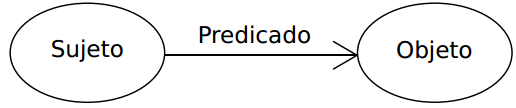
\includegraphics[width=12cm]{img/graficoRDF.png}
	\caption{Modelo de datos basado en grafo del estándar RDF}
	\label{fig:Modelo de datos basado en grafo del estándar RDF}
\end{figure}

\subsection{Ontologías}

La evolución del RDF en el ``Lenguaje de Ontologías Web'' (``Web Ontology Language'' - OWL, por sus siglas de acuerdo al término en idioma inglés) permite una descripción semántica más rica basada en Lógica Descriptiva \citep{Horrocks}. El OWL ha sido utilizado en varios escenarios específicos para la construcción de modelos de datos flexibles \citep{Agus,Munir,Franke2014,Sule2016}. 

El término ontología es utilizado con diferentes significados en diferentes comunidades. Su origen se encuentra en la filosofía y son utilizadas para estudiar la naturaleza del ser y su existencia \citep{Gruber1993,Gomez-Perez2004}. En computación una definición ampliamente aceptada fue formulada por \cite{Gruber1993} el cual afirma que \textit{una ontología es una especificación explícita de una conceptualización}. Años más tarde \cite{Studer1998} se basan en este concepto y lo extienden, afirmando que \textit{una ontología es una especificación formal y explícita de una conceptualización compartida}. Según \cite{Studer1998} una ontología:

\begin{itemize}
\item Es explícita porque define los conceptos, propiedades, relaciones, funciones, axiomas y restricciones que la componen.
\item Es formal porque es legible e interpretable por computadoras.
\item Es una conceptualización porque es un modelo abstracto y una vista simplificada de los elementos reales que representa.
\item Es compartida porque se ha arribado previamente a un consenso sobre la información y es aceptada por un grupo de expertos.
\end{itemize}

\cite{Staab2009} afirman que existen cuatro tipos diferentes de ontologías a diferentes niveles de granularidad. En un nivel superior se encuentran las ontologías fundacionales, las cuales capturan conceptos generales independientes de un dominio específico. En un segundo nivel de abstracción se encuentran las ontologías de dominio, las cuales modelan conceptos y relaciones que son relevantes para un dominio específico. En estas ontologías se suelen utilizar los términos de la ontologías fundacionales.

Otro tipo de ontología son las ontologías de tareas, las cuales describen conceptos de una tarea en específico. A un nivel más bajo de abstracción se encuentran las ontologías de aplicaciones. Estas combinan ontologías de dominio y ontologías de tareas extendiéndolas con nuevos conceptos y relaciones más específicos \citep{Staab2009}.

\cite{Gruber1993} y \cite{Gomez-Perez2004} proponen que las ontologías se modelen utilizando cinco tipos de componentes: clases, relaciones, funciones, instancias y axiomas formales. Las \textbf{clases} representan conceptos que pueden ser abstractos o no. Las clases de una ontología comúnmente se organizan en taxonomías a través de las cuales se pueden aplicar mecanismos de herencia.

Las \textbf{relaciones} representan tipos de asociaciones entre conceptos del dominio. Formalmente se pueden definir como cualquier subconjunto del producto de $n$ conjuntos, esto es $R \subset C_1 \,\times \,C_2 \,\times \ldots \times \,C_n$. Las ontologías con frecuencia poseen relaciones binarias, donde el primer argumento es conocido como el dominio y el segundo como el rango \citep{Gomez-Perez2004}.

Las \textbf{funciones} son un caso especial de relaciones donde el $n$-ésimo elemento de la relación es único para los $n-1$ elementos precedentes, es decir, $F: C_1 \,\times \,C_2 \,\times \ldots \times \,C_{n-1} \rightarrow C_n$ \citep{Gomez-Perez2004}.

Las \textbf{instancias} se utilizan para representar los individuos en una ontología \citep{Gomez-Perez2004}.

Según \cite{Gruber1993} los axiomas formales sirven para modelar sentencias que siempre son verdaderas. Normalmente se usan para representar conocimiento que no puede ser definido formalmente por otros componentes. Además, los axiomas formales se usan para verificar la consistencia de la ontología en sí misma o la consistencia del conocimiento almacenado en una base de conocimiento \citep{Gomez-Perez2004}. 

\subsection{Metodologías para el desarrollo de ontologías}

La Ingeniería Ontológica es la disciplina que estudia los principios, métodos y herramientas para crear y mantener ontologías. Una metodología de Ingeniería Ontológica proporciona el aspecto metodológico del desarrollo de ontologías. Con el objetivo de asistir a los ingenieros ontológicos y a los expertos de dominio en la construcción de ontologías se han desarrollado varias metodologías para la Ingeniería Ontológica \citep{Iqbal2013}.

Un análisis en profundidad de las principales metodologías para el desarrollo de ontologías es realizado por \cite{Iqbal2013}, estos autores proponen ocho criterios para la comparación de metodologías que se detallan a continuación.

\textbf{Criterio 1. Tipo de desarrollo}

La literatura revela que las metodologías para el desarrollo de ontologías pueden dividirse en tres categorías fundamentales: modelos basados en etapas, modelos de prototipos evolutivos y guías; dependiendo del tipo de modelo de desarrollo que siguen. Los diferentes enfoques tienen sus aspectos positivos y negativos. Las metodologías basadas en etapas pueden ser factibles en escenarios donde el propósito y los requerimientos están claramente definidos. Por el contrario, los prototipos evolutivos pueden ser la mejor elección cuando los requerimientos no están claramente definidos desde el inicio y es necesario refinar la ontología con el paso del tiempo. Las guías mayormente se enfocan en hacer sugerencias útiles, recomendar reglas y técnicas con el objetivo de tomar mejores decisiones en lugar de enfocarse en el modelo de desarrollo en sí.

\textbf{Criterio 2. Soporte para la construcción colaborativa}

Las ontologías pueden construirse tanto de forma aislada como colaborativamente. El soporte para la construcción colaborativa permite a diferentes miembros del equipo de desarrollo de ontologías trabajar en una misma ontología a la vez. Los miembros del equipo de desarrollo pueden estar dispersos geográficamente sin afectar la eficiencia del proyecto. 

\textbf{Criterio 3. Soporte para re-utilización}

El desarrollo de ontologías es una tarea costosa en tiempo y esfuerzo. Con el fin de economizar estos factores la noción de ontologías re-utilizables ha cobrado fuerzas a lo largo del tiempo. Las metodologías que soportan la re-utilización les permiten a los equipos de desarrollo de ontologías hacer uso de ontoloogías ya existentes reduciendo el tiempo y esfuerzo empleado en el desarrollo. El ahorro del tiempo les permite a los ingenieros enfocarse en los defectos presentes en las ontologías existentes, mejorando su calidad. 

\textbf{Criterio 4. Soporte para interoperabilidad}

Las ontologías de dominio que se desarrollen utilizando metodologías que soporten la interoperabilidad, proveerán a los sistemas que las usen de los mismos conceptos de alto nivel, por lo que les será más fácil comunicarse y compartir la información que gestionan entre sí.

\textbf{Critero 5. Grado de dependencia de la aplicación}

Diferentes metodologías durante el proceso de desarrollo pueden adoptar diferentes enfoques en cuanto a la dependencia de una aplicación. Una metodología puede optar por uno de tres escenarios: dependiente de la aplicación (la ontología se desarrolla enfocada en la base de conocimiento para una aplicación específica), semi-independiente de la aplicación (la ontología se desarrolla teniendo en cuenta posibles escenarios de aplicación durante la etapa de especificación) e independiente de la aplicación (la ontología se desarrolla sin enfocarse en un sistema en particular).

\textbf{Criterio 6. Recomendación del ciclo de vida}

El ciclo de vida de una ontología identifica el conjunto de etapas por las que pasa una ontología durante su vida. Varias metodologías no recomiendan claramente un ciclo de vida.

\textbf{Criterio 7. Estrategias para la identificación de conceptos}

La identificación de los conceptos candidatos para la inclusión en la ontología es indudablemente un proceso crucial en el desarrollo de la misma. Existen técnicas para la identificación de conceptos, algunas de ellas utilizan un enfoque abajo - arriba, mientras que otras emplean un enfoque arriba - abajo y unas terceras el enfoque que siguen es del centro hacia afuera.

\textbf{Criterio 8. Nivel de detalle de la metodología}

Cada metodología comprende algunas actividades y técnicas para soportar el desarrollo de ontologías. El análisis de la literatura ha revelado la existencia de metodologías que no proveen suficientes detalles para el empleo de sus actividades y técnicas. Para propósitos de análisis, este trabajo clasificará las metodologías en tres grupos de acuerdo a este criterio: suficientes detalles, algunos detalles e insuficientes detalles. Las metodologías que no brindan detalles o estos son muy vagos se clasificarán como de insuficientes detalles. Por otra parte, las metodologías que no cubren completamente los detalles pero al menos proporcionan algunos detalles sobre sus actividades y técnicas se clasificarán como algunos detalles. Asimismo, las metodologías clasificadas como suficientes detalles proveen un razonable nivel de detalles sobre las actividades y técnicas que emplean, permitiendo al lector comprenderlas claramente. 

Una clasificación de las metodologías analizadas de acuerdo a los criterios anteriormente expuestos se brinda en la Tabla \ref{tab:tablaComparativa} tomada del trabajo de \cite{Iqbal2013}. Posterior al análisis de diferentes metodologías para el desarrollo de ontologías se decidió utilizar para el presente trabajo METHONTOLOGY ya que recomienda un ciclo de vida, es reutilizable y provee suficientes detalles sobre las técnicas y actividades empleadas en ella.

\begin{table*}[!ht]
\centering
\caption{Comparación de las metodologías analizadas.}
\label{tab:tablaComparativa}
%\begin{adjustbox}{angle=90}
\resizebox{\textwidth}{!}{%
\begin{tabular}{p {3,5cm} p {2cm} p {2cm} p {2cm} p {2cm} p {2cm} p {2cm} p {2cm} p {2cm}}
\hline 
Metodologías & Tipo de Desarrollo & Construcción colaborativa & Reutiliza & Dependiente de la aplicación & Ciclo de vida & Estrategias para identificar los conceptos & Nivel de detalle & ¿Interoperable? \\ 
\hline 
TOVE & Basada en etapas & No & Sí & Semi independiente & No & Media & Algunos detalles & No \\ 

\textit{Enterprise model approach} & Basada en etapas & No & Sí & Independiente & No & Media & Algunos detalles & No \\ 
 
METHONTOLOGY & Prototipo evolutivo & No & Sí & Independiente & Sí & Media & Suficientes detalles & No \\ 
 
KBSI IDEF5 & Prototipo evolutivo & No & Sí & Independiente & No & No es clara & Algunos detalles & No \\ 
 
Ontolingua & Desarrollo modular & Sí & Sí & Independiente & No & No es clara & Algunos detalles & Sí \\ 
 
KACTUS & Desarrollo modular & No & Sí & Dependiente & No & Estrategia arriba-abajo & Insuficientes detalles & No \\ 
 
PLINIUS & Basada en guías & No & No & Independiente & No & Estrategia abajo-arriba & Algunos detalles & No \\ 
 
ONIONS & Desarrollo modular basado en guías & No & No & Dependiente & No & No es clara & Insuficientes detalles & Sí \\ 
 
Mikrokosmos & Basada en guías & No & No & Dependiente & No & Estrategia basada en reglas & Algunos detalles & No \\ 
 
MENELAS & Basada en guías & No & No & Dependiente & No & Grafos de conceptos & Insuficientes detalles & No \\ 
 
SENSUS & No menciona preferencias & Sí & Sí & Semi independiente & No & Abajo-arriba & Algunos detalles & Sí \\ 
 
Cyc & Prototipo evolutivo & No & Sí & Independiente & No & No es clara & Algunos detalles & No \\ 
 
UPON & Prototipo evolutivo & No & Sí & Independiente & Sí & Media & Algunos detalles & No \\ 

Método 101 & Prototipo evolutivo & No & Sí & Independiente & No & Consenso del desarrollador & Algunos detalles & No \\ 

On-To-Knowledge & Prototipo evolutivo & No & No & Dependiente & Sí & Media & Algunos detalles & No \\ 
\hline 
\end{tabular}} 
%\end{adjustbox}
\end{table*}

\subsection{Datos Enlazados Abiertos}
Los Datos Enlazados Abiertos son un conjunto de principios y buenas prácticas para la publicación de datos en la Web. Estos datos pueden estar dispersos geográficamente y pertenecer a una o varias organizaciones. En este sentido \cite{Berners-Lee2006} propone cuatro principios:

\begin{enumerate}
\item Utilizar URIs como nombres para las cosas.

\item Utilizar URIs HTTP para que las personas puedan buscar esos nombres.

\item Cuando alguien busca una URI, proveer información útil por medio de los estándares.

\item Incluir vínculos a otras URIs para que se puedan descubrir más cosas.
\end{enumerate}

El primer principio propone el uso de URIs para identificar no solo documentos web y contenido digital, sino que sirva además para referenciar a objetos del mundo real y conceptos abstractos. El segundo principio propone el uso de URIs basadas en el protocolo HTTP para identificar objetos y conceptos abstractos, posibilitando que estas URIs estén desreferenciadas sobre dicho protocolo y en cambio proporcionen una descripción del objeto o concepto identificado. El tercer principio propone el uso del modelo de datos RDF para publicar datos estructurados en la Web. El cuarto principio propone el uso de enlaces para enlazar no solo documentos web, sino cualquier tipo de recurso \citep{Hidalgo-Delgado2015}.

\section{Integración de datos}
Actualmente la existencia, competitividad y rentabilidad de diversas compañías depende de los flujos de datos. Sin embargo, la variedad de fuentes, tipos y volúmenes de datos ha vuelto más complejo el proceso de encontrarlos \citep{AloomaInc.2017}. La integración de datos se refiere a las técnicas involucradas en combinar los datos almacenados en diferentes ubicaciones en una vista común integrada \citep{Michel2017}. La disponibilidad de recursos de información heterogéneos y distribuidos ha conducido a considerar aproximaciones para la integración de datos en los que fuentes de datos independientes puedan participar en federaciones virtuales de datos. Mientras que los almacenes de datos son repositorios rígidos controlados por las premisas de una sola compañía, las nuevas necesidades de información deben acomodarse a la adición oportuna de nuevas fuentes de datos provenientes de instituciones independientes.

Por otra parte, la semántica de los datos almacenados en ocasiones no es descrita por los esquemas de bases de datos. Hasta cierto punto la semántica implícita de los datos se puede inferir a partir de las restricciones de integridad o patrones de diseño de bases de datos comunes, pero la semántica adicional se encuentra codificada en las aplicaciones que consumen las fuentes de datos. Además, frecuentemente los esquemas de bases de datos se optimizan por cuestiones de rendimiento, resultando en una mezcla de la semántica de los datos con aspectos técnicos. Por estas razones, los métodos utilizados para la integración de datos en la Web deben poseer la capacidad de capturar y compartir conceptualizaciones formales comunes en una manera explícita 
procesable por computadoras. Esto convencionalmente se logra por medio de la utilización de vocabularios controlados, tesauros y ontologías.

\subsection{Principios para la integración de datos}
Convencionalmente, un sistema para la integración de datos $\Psi$ se denota por la tupla $<\Gamma , \Upsilon , \Sigma>$ donde:

\begin{itemize}
\item $\Gamma$ es el esquema global utilizado para representar la vista unificada.
\item $\Upsilon$ son las fuentes de datos representadas por el conjunto de esquemas locales $\upsilon_1 , \cdots , \upsilon_n$.
\item $\Sigma$ especifica las correspondencias entre los conceptos de los esquemas locales y los conceptos del esquema global.
\end{itemize}

Dependiendo de los lenguajes de modelado utilizados para definir los esquemas locales y globales, los conceptos pueden ser clases de una ontología, tablas de una base de datos, objetos, entre otros.

Un sistema para la integración de datos responde a consultas formuladas en términos del esquema global $\Gamma$ reformulándolas en las consultas correspondientes sobre las fuentes de datos $\upsilon_1 , \cdots , \upsilon_n$ por medio de la información almacenada en $\Sigma$. Con respecto a la forma en que se expresan los mapeos se han propuesto dos enfoques principales: el enfoque ``Global-como-Vista'' (``Global-as-View'' - GAV, por sus siglas de acuerdo al término en idioma inglés), en el que el esquema global se expresa en términos de consultas (o vistas) sobre los esquemas locales; mientras que en el enfoque ``Local-como-Vista'' (``Local-as-View'' - LAV, por sus siglas de acuerdo al término en idioma inglés), los esquemas globales se expresan en términos de consultas (o vistas) sobre el esquema global. Estos enfoques han sido abundantemente descritos en la literatura \citep{Doan:2012:PDI:2401764,Lenzerini:2002:DIT:543613.543644}.

Variados son los sistemas propuestos para la integración de datos basados en RDF, unos en forma de motores de consultas federados sobre SPARQL \citep{Schwarte:2011:FOT:2063016.2063055,Gorlitz:2011:SSE:2887352.2887354,Corby:2012:KVI:2457524.2457672,macina2016sparql} y otros como fragmentos de Datos Enlazados \citep{VERBORGH2016184}. Sin embargo, los enfoques de estos sistemas no se pueden clasificar claramente como GAV o LAV porque sus objetivos son producir planes de consultas eficientes sobre fuentes de datos distribuidas que soportan SPARQL sin la mediación de un esquema.

\subsection{Acceso e Integración de Datos Basado en Ontologías}
El ``Acceso a Datos Basado en Ontologías'' (``Ontology-based Data Access'' - OBDA, por sus siglas de acuerdo al término en idioma inglés) es un dominio de la Integración de Datos que propone la utilización de ontologías para crear una capa conceptual formal; en esta capa la ontología representa el dominio de los datos almacenados en la fuente de datos y el mapeo describe las relaciones entre la ontología y la fuente de datos \citep{Calvanese:2015:SOY:2991147.2991152,KHARLAMOV20173}. \cite{Tabares-Martin2016} definen formalmente un sistema OBDA como una tupla \( \Omega = <\tau,\sigma,\mu> \) donde:

\begin{itemize}
 	\item \(\tau\) es la parte terminológica de la ontología. Se consideran ontologías basadas en Lógica Descriptiva, por lo que $\tau$ es una TBox según la Lógica Descriptiva.
 	\item $\sigma$ es el conjunto de fuentes de datos.
 	\item $\mu$ es un conjunto de mapeos, cada uno de la forma $\Phi(x) \leftarrow \Xi(x)$ donde:
 	\begin{itemize}
 		\item[•] $\Phi(x)$ es una consulta sobre $\sigma$, retornando las tuplas de valor para $x$.
 		\item[•] $\Xi(x)$ es una consulta sobre $\tau$ cuyas variables libres provienen de $x$.
 	\end{itemize}
\end{itemize}

La ontología en el paradigma OBDA provee un punto de acceso único para un acceso a datos semántico destinado a los consumidores de datos, a la vez que permite exportar los datos de las fuentes integradas en un formato semántico o ejecutar consultas en términos de un modelo conceptual orientado al usuario que lo abstraen de los detalles a nivel de implementación que comúnmente se encuentran en los esquemas de bases de datos \citep{KHARLAMOV20173}. Por otra parte, los expertos en el dominio son capaces de expresar las necesidades de información en sus propios términos sin conocimiento previo sobre la forma en que están estructurados los datos en la fuente, a la vez que reciben las respuestas a sus consultas en los términos definidos en la ontología.

La ``Integración de Datos Basada en Ontologías'' (``Ontology-based Data Integration'' - OBDI, por sus siglas de acuerdo al término en idioma inglés) es un caso más general de OBDA en el cual las organizaciones gestionan de forma integrada diferentes fuentes de datos por medio del paradigma OBDA. La OBDI se ha utilizado en trabajos como los descritos por \cite{Calvanese2016,Daraio2016,Kharlamov:2016:OIS:2882903.2899385}

\section{Conclusiones parciales}
El objetivo que persigue este trabajo es desarrollar un método con componentes semánticos que permita la integración en una aplicación informática de datos relativos al Control de Autoridades almacenados de forma heterogénea. En este capítulo se abordó el Control de Autoridades realizando un análisis histórico de su desarrollo. Posteriormente se analizaron diferentes elementos que forman parte de las tecnologías de la Web Semántica y que posibilitan describir semánticamente los datos almacenados en fuentes estructuralmente heterogéneas. Luego se examinaron principios para la integración de datos, haciendo énfasis en la integración semántica de datos.

Al realizar la revisión bibliográfica respectiva al estado del arte de la temática se evidenciaron diferentes aproximaciones que posibilitan la integración semántica de datos, siendo la Integración de Datos Basada en Ontologías una de las más promisorias. Sin embargo, a pesar de que se describen los elementos que intervienen en la OBDI, en la literatura revisada no se especifica un método para llevarla a cabo.








